\begin{figure}[t]
\centering
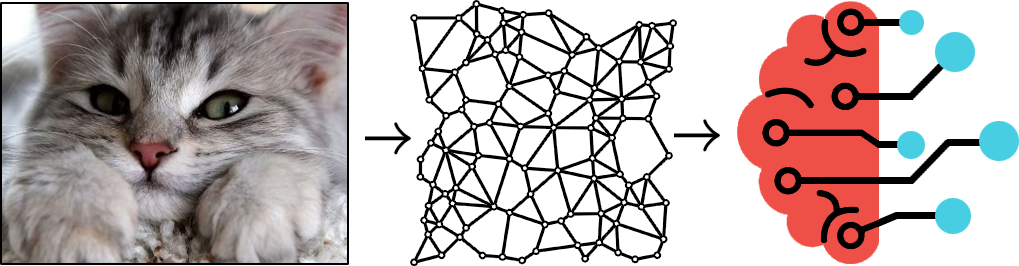
\includegraphics[width=\textwidth]{bilder/problemstellung.png}
\caption[Problemstellung]{Illustration der verfolgten Problemstellung in dieser Arbeit.
Bilder werden für ihre Eingabe in ein neuronales Netz zuvor in eine korrespondierende Graphrepräsentationen konvertiert, auf denen gelernt wird.}
\label{fig:problemstellung}
\end{figure}
